\documentclass[../thesis.tex]{subfiles}
\begin{document}
\section{Lý do lựa chọn đề tài}
\subsection{Chương trình nông thôn mới là một trong những chương trình có tính ảnh hưởng quốc gia, với mục đích thúc đẩy phát triển nông nghiệp và nông thôn.}
Chương trình mục tiêu quốc gia về xây dựng nông thôn mới được quy định trong Quyết định số 800/QĐ-TTG của Thủ tướng Chính phủ : Phê duyệt Chương trình mục tiêu Quốc gia về xây dựng nông thôn mới giai đoạn 2010 - 2020 là “một chương trình tổng thể về phát triển kinh tế - xã hội, chính trị và an ninh quốc phòng”, có phạm vi áp dụng là nông thôn trên địa bàn toàn quốc từ 2010 đến 2020. Mô hình nông thôn mới được Ban Bí thư lựa chọn thí điểm tại 11 xã khắp toàn quốc, trong đó có xã Thuỵ Hương huyện Chương Mỹ. Những bài học được rút ra trong quá trình thí điểm 11 xã này sẽ được điều chỉnh và rút kinh nghiệm ở các trường hợp sau.\\ 
Bởi vậy, có thể nhận định các chính sách quy hoạch xây dựng NTM tại xã Thụy Hương Chương Mỹ có hai tính chất: (1) tính nguyên gốc: đại diện cho ảnh hưởng của chính sách NTM thời đầu (2) tính ảnh hưởng: trở thành bài học cho việc  phát triển NTM trên toàn quốc gia Việt Nam.
\subsection{Nhu cầu định hướng không gian kiến trúc cảnh quan nông thôn trong giai đoạn mới}
Tham luận “Triển khai Quy hoạch Xây dựng Nông thôn gắn với Chương trình MTQG Xây Dựng Nông Thôn Mới” của BXD tại “Hội nghị tổng kết 10 năm thực hiện Chương trình mục tiêu quốc gia xây dựng nông thôn mới giai đoạn 2010-2020” đã đề ra các định hướng về Quy hoạch xây dựng nông thôn mới như sau:
- \say{\textit{Định hướng không gian quy hoạch cảnh quan nông thôn cần chú trọng đến bảo tồn, chỉnh trang các không gian làng, xã vốn có trước đây. Căn cứ điều kiện địa lý của từng vùng, mỗi địa phương để lập quy hoạch, xây dựng cảnh quan bảo đảm phù hợp, nhưng vẫn tạo nên sự hài hòa và thân thiện với môi trường.\\
- Xác định các khu vực cảnh quan trọng tâm để tạo điểm nhấn và nét độc đáo riêng có đối với mỗi xã nông thôn mới nâng cao cũng như nông thôn mới kiểu mẫu.\\
- Gắn kết các thị trấn, thị tứ, điểm dân cư tập trung trên địa bàn huyện hoặc liên huyện với các điểm sản xuất, dịch vụ từ nông nghiệp. Tạo điều kiện cho quá trình đô thị hoá tại chỗ, phát triển dân cư phi nông nghiệp trên địa bàn cấp huyện, xã.\\
- Định hướng mạng lưới hạ tầng khung phục vụ sản xuất và liên kết giữa địa bàn sản xuất với khu dân cư, giữa các khu dân cư với nhau trên địa bàn cấp huyện.\\
- Có định hướng bảo vệ và gìn giữ những nét truyền thống của thôn bản xưa, tạo dựng cảnh quan xanh - sạch - đẹp phù hợp với điều kiện tự nhiên của từng thôn, xã. Theo Luật Kiến trúc mới được Quốc hội ban hành ngày 13/6/2019, tại khoản 2 điều 11 thì kiến trúc nông thôn phải đáp ứng yêu cầu sau:\\ (1) Bảo đảm kế thừa giá trị kiến trúc truyền thống, bản sắc văn hóa dân tộc; (2) Ưu tiên sử dụng vật liệu xây dựng địa phương và giải pháp kỹ thuật xây dựng tiên tiến; (3) Bảo đảm tiêu chuẩn về nhà ở, không gian sống, không gian văn hóa phù hợp với điều kiện tự nhiên, tập quán sinh hoạt, thuần phong mỹ tục của cộng đồng các dân tộc; (4) Đối với khu vực thường xảy ra thiên tai, khuyến khích áp dụng mẫu thiết kế kiến trúc cho công trình công cộng và nhà ở nông thôn bảo đảm yêu cầu về thích ứng với biến đổi khí hậu và phòng, chống thiên tai.}}\\[0.25cm]
Có thể nhận thấy tham luận đã gợi mở về hai định hướng phát triển nông thôn, (1) một là hài hòa cảnh quan, đưa những yếu tố văn hóa, truyền thống, di sản vào không gian nông thôn vốn có, khai thác nét đặc trưng địa phương; (2) hai là phát triển hạ tầng làm cơ sở đô thị hóa trong tương lai, Việc ra đời Luật Kiến trúc đã làm rõ ràng hơn khái niệm về “Kiến trúc nông thôn”. Từ đó, có thể nhận thấy nhu cầu về những nghiên cứu định hướng Quy hoạch Kiến trúc Cảnh quan nông thôn thực tiễn trong giai đoạn mới là cấp thiết.
\subsection{Vai trò không gian kiến trúc cảnh quan trong quá trình phát triển nông thôn
}
\section{Mục đích nghiên cứu}
\subsection{Mục đích}
Đánh giá Sự biến đổi không gian kiến trúc cảnh quan qua các chính sách phát triển Nông thôn mới trong thực tiễn tại 3 thôn Chúc Đồng,Trung Tiến, Tân Mỹ dưới quan điểm về phát triển điểm dân cư nông thôn bền vững, đáng sống. Từ đó, đưa ra  khuyến nghị đối với khu vực cũng như những xã nông thôn ĐBCTSH có bối cảnh tương tự để phát triển.
\subsection{Mục tiêu}
Để thực hiện việc đánh giá sự biến đổi không gian kiến trúc cảnh quan dưới ảnh hưởng \textit{Các chính sách MTQG Chương trình phát triển Nông thôn mới có liên quan tới phát triển không gian kiến trúc cảnh quan} tại khu vực, luận văn thực hiện ba mục tiêu cụ thể:
\begin{enumerate}
	\item \textbf \textbf{Hệ thống hoá} Các chính sách MTQG Chương trình phát triển Nông thôn mới có liên quan tới phát triển không gian kiến trúc cảnh quan từ 2009-2020: Thống kê các tiêu chí có ảnh hưởng tới phát triển không gian kiến trúc cảnh quan.
	\item Nhận diện \textbf{sự biến đổi không gian kiến trúc cảnh quan} dưới ảnh hưởng các các chính sách NTM liên quan trong thực tế: Thông qua khảo sát xã hội học, quan sát thực tiễn, so sánh đối chiếu bản đồ địa chính, bản đồ viễn thám nhằm đưa ra các nhận định về sự biến đổi không gian kiến trúc cảnh quan
	\item \textbf{Thành lập bảng tiêu chí} trên cơ sở khảo sát xã hội học, tổng hợp từ các bài học trên thế giới và trong nước, quan điểm của các chuyên gia. Đối chiếu bảng tiêu chí với cụ thể trường hợp tại khu vực nghiên cứu.
	\item Từ đó, đưa ra dự báo, khuyến nghị, đề xuất giải pháp để phát triển không gian trong giai đoạn mới
\end{enumerate}
\section{Đối tượng và phạm vi nghiên cứu}
Sự biến đổi không gian kiến trúc cảnh quan tại 3 thôn Chúc Đồng,Trung Tiến, Tân Mỹ trong quá trình phát triển NTM, cụ thể:
\begin{enumerate}
    \item \textbf{Sử dụng đất:} So sánh các bản vẽ hiện trạng sử dụng đất, bản đồ địa chính, quy hoạch sử dụng đất qua các giai đoạn (Trước giai đoạn NTM, Lập quy hoạch 2009 và điều chỉnh quy hoạch 2017) để nhận diện những thay đổi được đề xuất. Đồng thời đối chiếu với thực tiễn thông qua khảo sát, phỏng vấn người dân, quan sát thực tế tại khu vực, tư liệu viễn thám và tư liệu truyền thông để trả lời câu hỏi: Những biến đổi không gian kiến trúc cảnh quan đã đem lại ảnh hưởng tích cực/ tiêu cực nào?
    \item \textbf{Phát triển không gian:} Xác định cấu trúc không gian và tiến trình phát triển không gian của khu vực thông qua các bản đồ, khảo sát thực địa và phỏng vấn người dân khu vực, so sánh đối chiếu các đề xuất định hướng phát triển không gian có phù hợp với hoàn cảnh, văn hóa địa phương chưa. Những không gian ấy có an toàn, thuận tiện, thẩm mĩ không?
    \item \textbf{Phát triển hạ tầng:} Đánh giá vai trò của hạ tầng đối với hình thái cấu trúc không gian kiến trúc cảnh quan khu vực. Đồng thời,những đề xuất phát triển hạ tầng kỹ thuật (giao thông, điện, nước) và hạ tầng xanh(cây xanh, cảnh quan) có đáp ứng được nhu cầu sinh hoạt thực tế của người dân (di chuyển, lao động, giải trí) hay không?
\end{enumerate}
\section{Câu hỏi nghiên cứu}
Ba câu hỏi nghiên cứu tập trung:
\begin{enumerate}
    \item Những chính sách nào trong phát triển NTM ảnh hưởng tới phát triển không gian kiến trúc cảnh quan?
    \item Không gian kiến trúc cảnh quan hiện hữu tại khu vực nghiên cứu đã được biến đổi như thế nào? Đánh giá những biến đổi ấy(phù hợp/ chưa phù hợp/ chưa đáp ứng).
    \item Những tác động nào có thể làm nhằm cải thiện KGKTCQ khu vực nghiên cứu.
    \item Những điều gì có thể rút ra về phát triển KGKTCQ NTM sau bài học tại khu vực nghiên cứu?
\end{enumerate}

%table
\begin{landscape}
\begin{figure}[ht!]
\caption{Khung nghiên cứu luận văn}
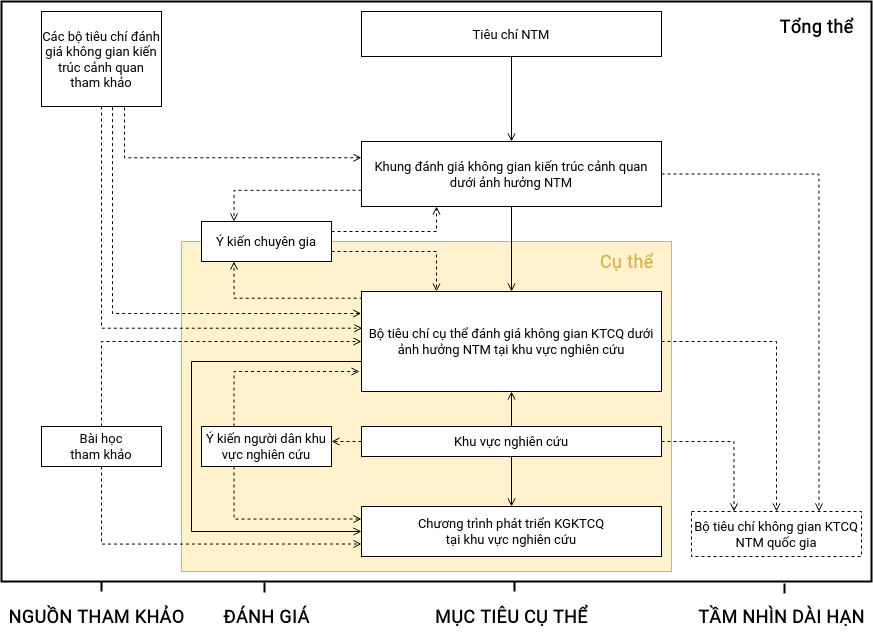
\includegraphics[width=21cm]{Graphic/index.png}
\end{figure}
\end{landscape}

\end{document}